\chapter{Results}

\label{chapter:results}

In this chapter, we focus on summarizing the results of our aforementioned
methodologies which we described to answer our three research questions. We
break this results chapter into three sections, with each section addressing one
research question. As a note, we do not dive deep into interpreting our results
but instead use this chapter to solely report on our results. We interpret the
results in greater detail in the next Discussion chapter.

\section{RQ1: Evaluating performance of SoPa++}

Following our methodologies, we conducted a grid-search training scheme where we
varied our patterns $P$ and $\tau$-threshold parameters. The variation in the
patterns hyperparameter $P$ resulted in three different \ac{sopa}++ model sizes;
specifically the small, medium and large model sizes as reported in Table
\ref{tab:model_types}. Along with ten random seed iterations for each grid
instance in our grid-search scheme, we ran a total of 150 models runs.

We start off by describing the training process for our \ac{sopa}++ models. Figure
\ref{fig:results_training} shows a visualization of the validation accuracy
against training updates in our grid-search training runs. Firstly, we
observe a trend that the larger models tend to have a higher validation accuracy
profiles compared to smaller models. Next, we observe that increasing the
$\tau$ value from 0.00 to 1.00 tends to decrease the overall validation accuracy
profile across all model sizes, albeit more drastically for smaller models than
larger models. Finally, we observe that the larger models tend to have an
earlier convergence window compared to the smaller models.

In regards to the evaluation of \ac{sopa}++ performance, we refer to Table
\ref{tab:results_evaluation} for a tabular summary of test accuracies across the
small, medium and large model sizes grouped by the various $\tau$-threshold
hyperparameters. Here, we can observe two trends. Firstly, the larger models
tend to have a higher mean test accuarcy. Secondly, the mean test accuarcy for
all models tends to decrease as the $\tau$-threshold increases. These trends are
also consistent with the validation accuracy trends in the previous section. The
best performing models for each model size are those where $\tau$=0.00.

\begin{figure}[t!]
  \centering
  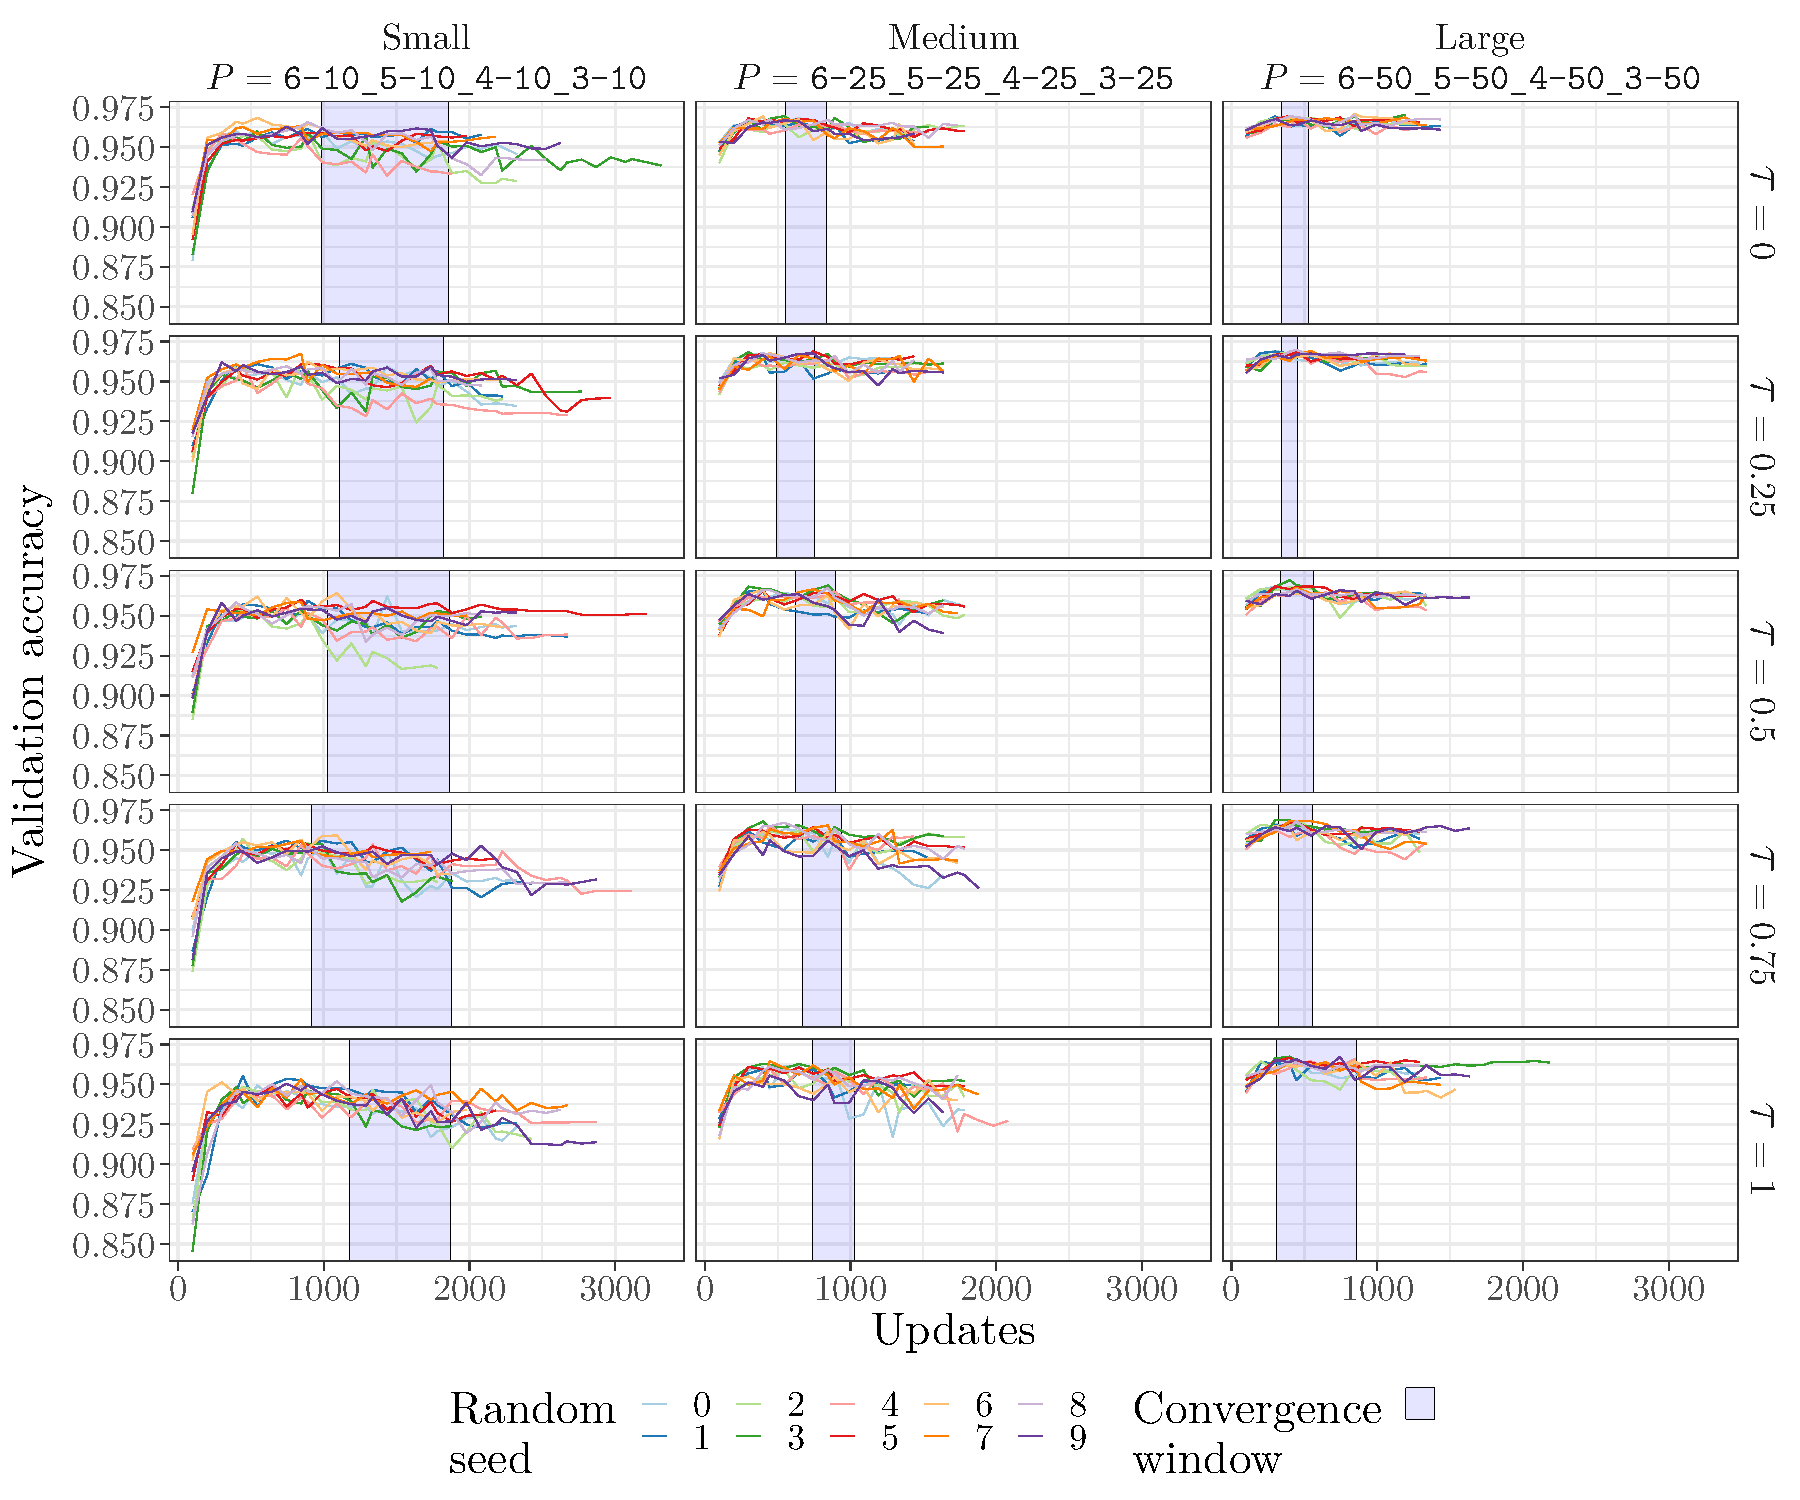
\includegraphics[width=14cm]{pdfs/generated/train_spp_grid_1618061447.pdf}
  \caption{Visualization of validation accuracy against number of training
    updates grouped by patterns $P$ and $\tau$-threshold hyperparameters; the
    different coloured lines represent random seed iterations with a
    specific initial random seed}
  \label{fig:results_training}
\end{figure}

\begin{table}[t!]
  \centering \def\arraystretch{1.3}
  \small
  \begin{tabular}{lllllll}
    \toprule
    && \multicolumn{5}{c}{Accuracy in $\%$ with mean $\pm$ standard-deviation} \\
    \cline{3-7} \\[-15pt]
    Size & Parameters & $\tau$=0.00 & $\tau$=0.25 & $\tau$=0.50 & $\tau$=0.75 & $\tau$=1.00 \\
    \midrule
    Small & 1,260,292 & \bm{$97.6 \pm 0.2$} & 97.6 $\pm$ 0.2 & 97.3 $\pm$ 0.2 & 97.0 $\pm$ 0.3 & 96.9 $\pm$ 0.3 \\
    Medium & 1,351,612 & \bm{$98.3 \pm 0.2$} & 98.1 $\pm$ 0.1 & 98.0 $\pm$ 0.2 & 97.9 $\pm$ 0.1 & 97.7 $\pm$ 0.1  \\
    Large & 1,503,812 & \bm{$98.3 \pm 0.2$} & 98.3 $\pm$ 0.2 & 98.2 $\pm$ 0.2 & 98.1 $\pm$ 0.2 & 98.0 $\pm$ 0.2 \\
    \bottomrule
  \end{tabular}
  \caption{Test accuracies of the SoPa++ models grouped by model sizes and
    $\tau$-threshold hyperparameters; mean accuracies and standard deviations were
    calculated across random seed iterations; bold scores show best performing
    model for each model size}
  \label{tab:results_evaluation}
\end{table}

\section{RQ2: Evaluating explanations by simplification}

\begin{figure}[t!]
  \centering
  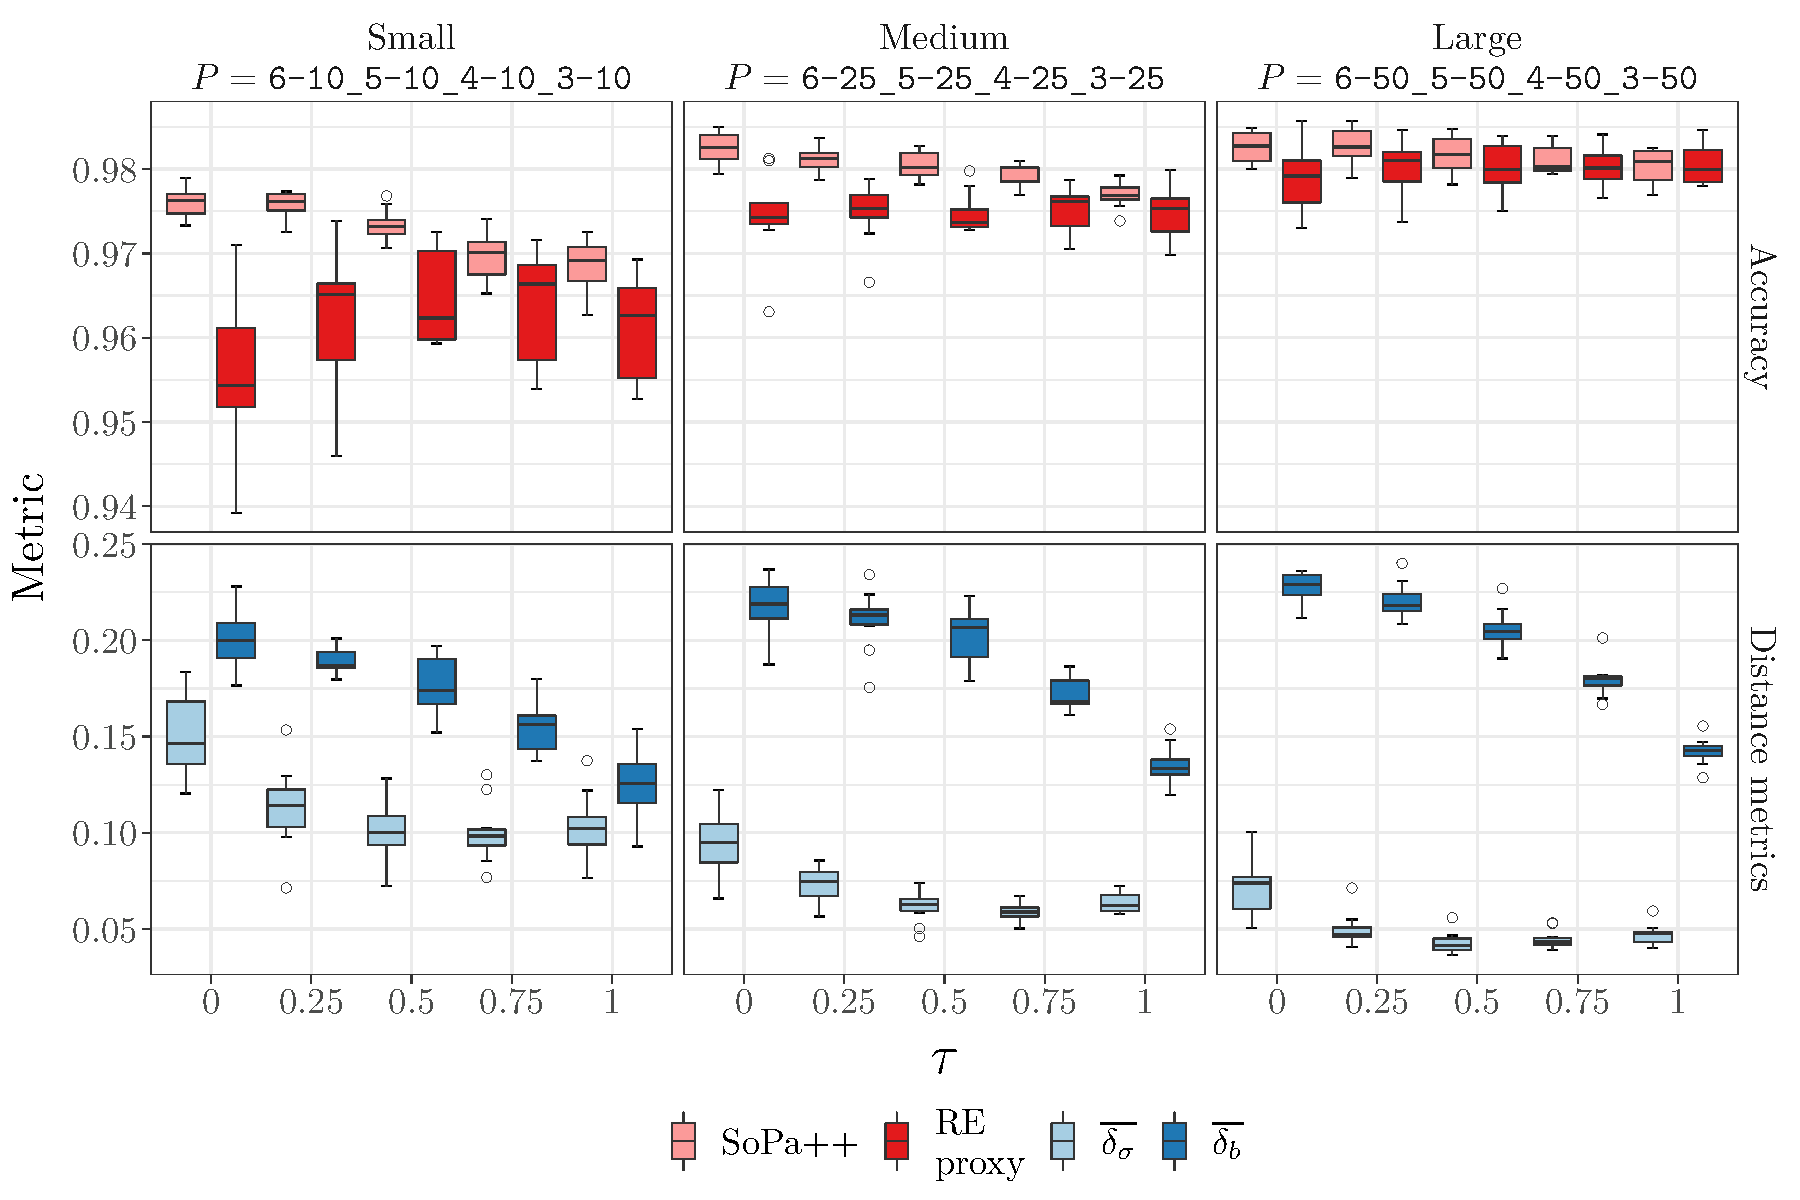
\includegraphics[width=14cm]{pdfs/generated/evaluate_spp_grid_1618059389.pdf}
  \caption{Visualization of accuracy and model-pair distance metrics against the
    $\tau$-threshold hyperparameter grouped by the patterns
    hyperparameter $P$}
  \label{fig:explain_evaluate}
\end{figure}

\begin{table}[t!]
  \centering \def\arraystretch{1.3}
  \small
  \begin{tabular}{lllllll}
    \toprule
    && \multicolumn{5}{c}{Accuracy in $\%$ with mean $\pm$ standard-deviation} \\
    \cline{3-7} \\[-15pt]
    Size & Model & $\tau$=0.00 & $\tau$=0.25 & $\tau$=0.50 & $\tau$=0.75 & $\tau$=1.00 \\
    \midrule
    Small & SoPa++ & 97.6 $\pm$ 0.2 & 97.6 $\pm$ 0.2 & 97.3 $\pm$ 0.2 & \bm{$97.0 \pm 0.3$} & 96.9 $\pm$ 0.3 \\
    & \ac{re} proxy & 95.5 $\pm$ 1.0 & 96.2 $\pm$ 0.8 & 96.5 $\pm$ 0.6 & \bm{$96.3 \pm 0.7$} & 96.1 $\pm$ 0.6 \\
    Medium & SoPa++ & 98.3 $\pm$ 0.2 & 98.1 $\pm$ 0.1 & 98.0 $\pm$ 0.2 & 97.9 $\pm$ 0.1 & \bm{$97.7 \pm 0.1$}  \\
    & \ac{re} proxy & 97.4 $\pm$ 0.5 & 97.5 $\pm$ 0.3 & 97.5 $\pm$ 0.2 & 97.5 $\pm$ 0.3 & \bm{$97.5 \pm 0.3$} \\
    Large & SoPa++ & 98.3 $\pm$ 0.2 & 98.3 $\pm$ 0.2 & 98.2 $\pm$ 0.2 & 98.1 $\pm$ 0.2 & \bm{$98.0 \pm 0.2$} \\
    & \ac{re} proxy & 97.9 $\pm$ 0.4 & 98.0 $\pm$ 0.3 & 98.0 $\pm$ 0.3 & 98.0 $\pm$ 0.2 & \bm{$98.1 \pm 0.2$} \\
    \bottomrule\\[-13pt]
    && \multicolumn{5}{c}{Metric in $\%$ with mean $\pm$ standard-deviation} \\
    \cline{3-7} \\[-15pt]
    Size & Metric & $\tau$=0.00 & $\tau$=0.25 & $\tau$=0.50 & $\tau$=0.75 & $\tau$=1.00 \\
    \midrule
    Small & $\overline{\delta_{\sigma}}$ & 15.0 $\pm$ 2.3 & 11.3 $\pm$ 2.2 & 10.0 $\pm$ 1.6 & \bm{$10.0 \pm 1.6$} & 10.3 $\pm$ 1.8 \\
    & $\overline{\delta_b}$ & 20.1 $\pm$ 1.5 & 18.9 $\pm$ 0.7 & 17.8 $\pm$ 1.5 & 15.5 $\pm$ 1.3 & \bm{$12.4 \pm 1.8$} \\
    Medium & $\overline{\delta_{\sigma}}$ & 9.5 $\pm$ 1.7 & 7.3 $\pm$ 0.9 & 6.1 $\pm$ 0.8 & \bm{$5.8 \pm 0.5$} & 6.3 $\pm$ 0.5  \\
    & $\overline{\delta_b}$ & 21.7 $\pm$ 1.5 & 21.0 $\pm$ 1.6 & 20.3 $\pm$ 1.5 & 17.2 $\pm$ 0.9 & \bm{$13.5 \pm 1.0$} \\
    Large & $\overline{\delta_{\sigma}}$ & 7.1 $\pm$ 1.5 & 5.0 $\pm$ 0.8 & \bm{$4.3 \pm 0.6$} & 4.5 $\pm$ 0.5 & 4.7 $\pm$ 0.5 \\
    & $\overline{\delta_b}$ & 22.7 $\pm$ 0.9 & 22.0 $\pm$ 1.0 & 20.6 $\pm$ 1.0 & 18.0 $\pm$ 0.9 & \bm{$14.2 \pm 0.7$} \\
    \bottomrule
  \end{tabular}
  \caption{Test accuracies and model-pair distances metrics of the SoPa++ and RE
    proxy models grouped by model sizes and $\tau$-thresholds; accuracies and
    standard deviations were calculated across random seed iterations; bold test
    accuracies show model pairs where mean accuracies are closest to one another;
    bold distance metrics indicate mean metrics that are closest to zero}
  \label{tab:explain_evaluate_performance}
\end{table}

Following our methodologies for evaluating explanations by simplification for
the \ac{sopa}++ model, we compare test set accuarcies and distance metrics between
\ac{sopa}++ and \ac{re} proxy model pairs. Figure \ref{fig:explain_evaluate} and Table
\ref{tab:explain_evaluate_performance} provide both a visualization and tabular
summary of all the aforementioned comparisons respectively. Overall, we can
observe three general trends. Firstly, we observe that \ac{sopa}++ and \ac{re} proxy test
accuracies tend to become converge towards one another as we increase the
$\tau$-threshold. Next, we can observe that \ac{re} proxy accuracies tend to be lower
than their \ac{sopa}++ counterparts during this convergence process; with a single
exception of the large model at $\tau=1.00$ where the \ac{re} proxy mean accuracy
exceeds that of \ac{sopa}++. Finally, we observe the general trend that both
$\overline{\delta_{\sigma}}$ and $\overline{\delta_b}$ become closer to zero as
we increase the $\tau$-threshold. This trend is consistently observed for
$\overline{\delta_b}$ but is not always the case for
$\overline{\delta_{\sigma}}$; which is minimized at $\tau$-threshold values of
0.50-0.75.

\section{RQ3: Interesting and relevant explanations}

\begin{figure}[t!]
  \centering
  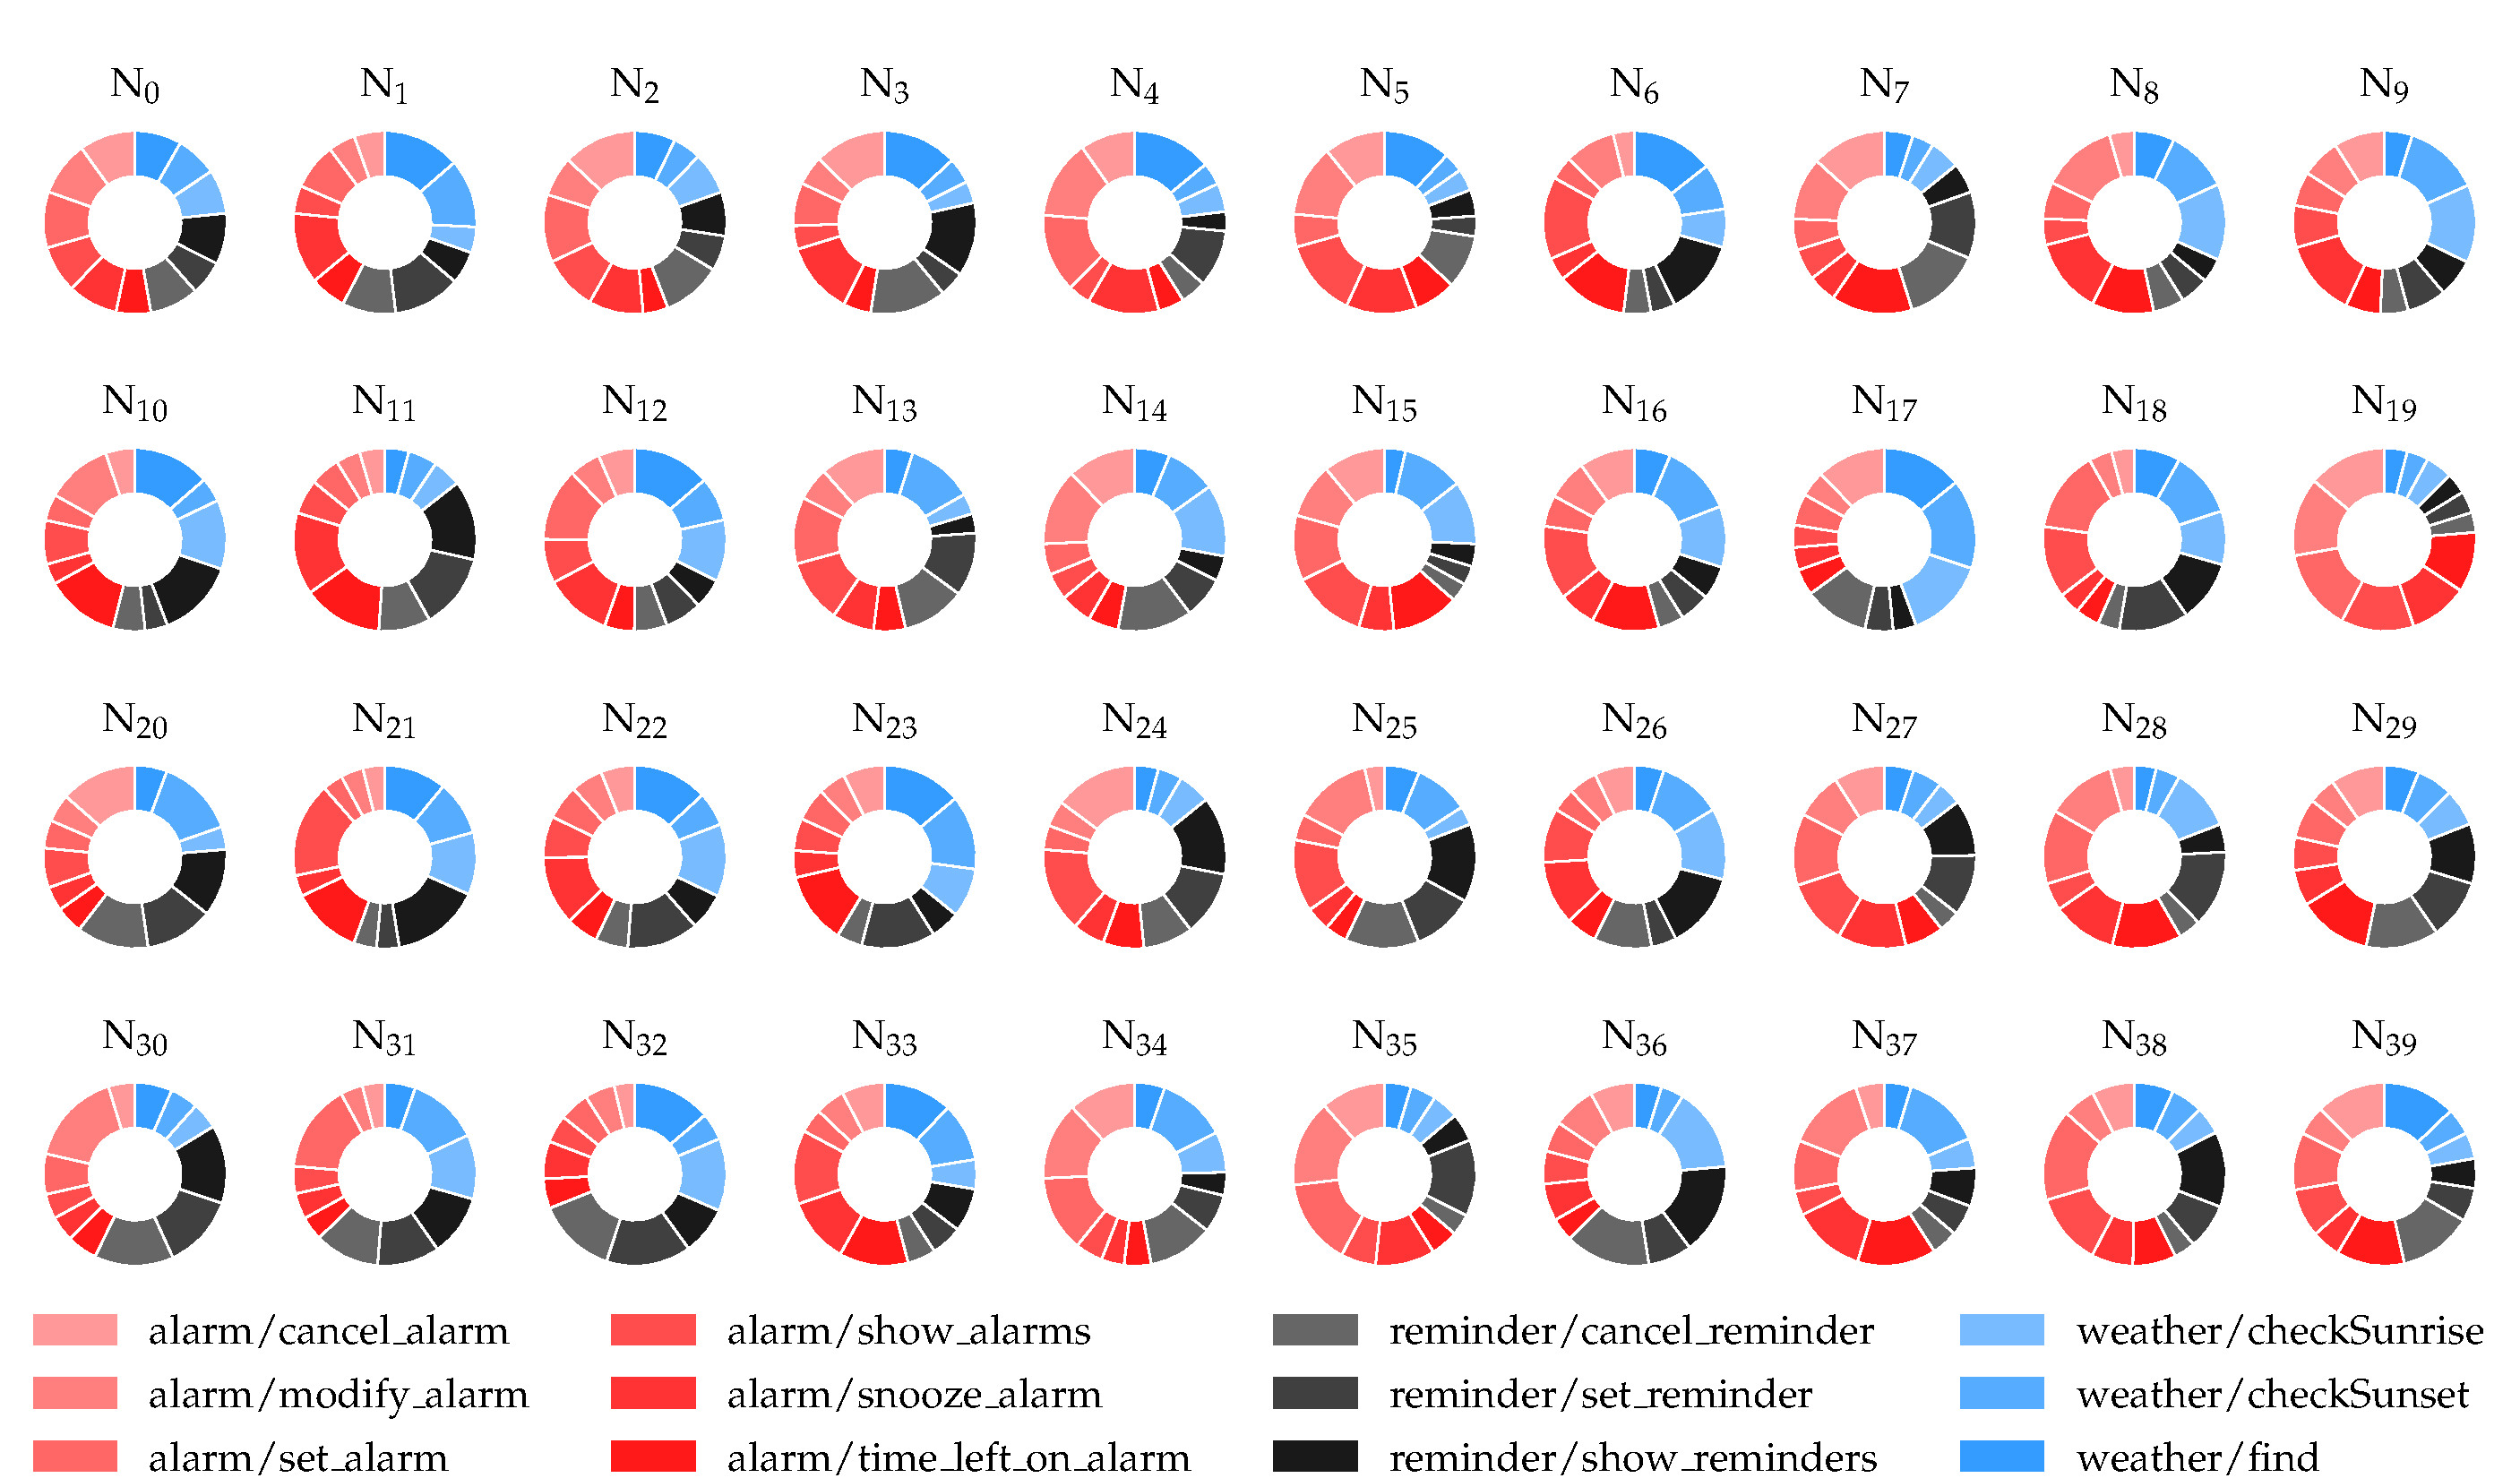
\includegraphics[width=14.5cm]{pdfs/generated/neurons_1618067685.pdf}
  \caption{Relative linear layer weights applied to TauSTE neurons for the best
    performing small RE proxy model with a test accuracy of 97.4$\%$}
  \label{fig:neuron_weights}
\end{figure}

Following our methologies to find interesting and relevant explanations on the
\ac{fmtod} data set, we start off by selecting a particular \ac{re} proxy model and
analyzing the relative linear weights applied to each \ac{tauste} neuron. For
simplicity and to minimize the number of \ac{tauste} neurons to visualize, we select
the best performing small \ac{re} proxy model with 40 \ac{tauste} neurons and a test set
accuracy of 97.4$\%$. Figure \ref{fig:neuron_weights} visualizes the relative
linear weights applied to each \ac{tauste} neuron in this \ac{re} proxy model. We can
observe that the relative linear weights are generally smoothly and evenly
distributed for each \ac{tauste} neuron among all the 12 \ac{fmtod} classes. That being
said, there exist salient \ac{tauste} neurons on which there are disproportionatey
large relative weights placed for certain domains compared to others. Examples
of these include neuron 19, 25 and 17 which place disproportionately large
relative weights on the alarm, reminder and weather domains respectively.

Next, we isolate the aforementioned salient \ac{tauste} neurons 19, 25 and 17 and we
sample ten "activating" regular expressions from the \ac{re} lookup layer
corresponding to these three neurons. We visualize these regular expressions as
strict linear-chain \ac{nfa} with $\omega$-transitions as shown in Figures
\ref{fig:regex_example_neuron_alarm}, \ref{fig:regex_example_neuron_reminder}
and \ref{fig:regex_example_neuron_weather} respectively. We can observe that
\ac{tauste} neurons 17 and 19 are used for capturing sub-strings of length 3, while
\ac{tauste} neuron 25 is used for capturing sub-strings of length 4. Next, we can
observe the segmentation of domain related information among the three neurons.
Finally, we can observe certain main-path transitions which show high degrees of
branching; which implies that these transitions were frequently utilized. While
we only sampled ten regular expressions per neuron from the \ac{re} lookup layer, it
should be noted that there exist many more regular expressions to explore.
Therefore, the following regular expressions only function as samples to provide
us with some notion of what kinds of regular expressions the \ac{sopa}++ and \ac{re} proxy
models captured as important.

\newpage

\begin{figure}[t!]
  \centering 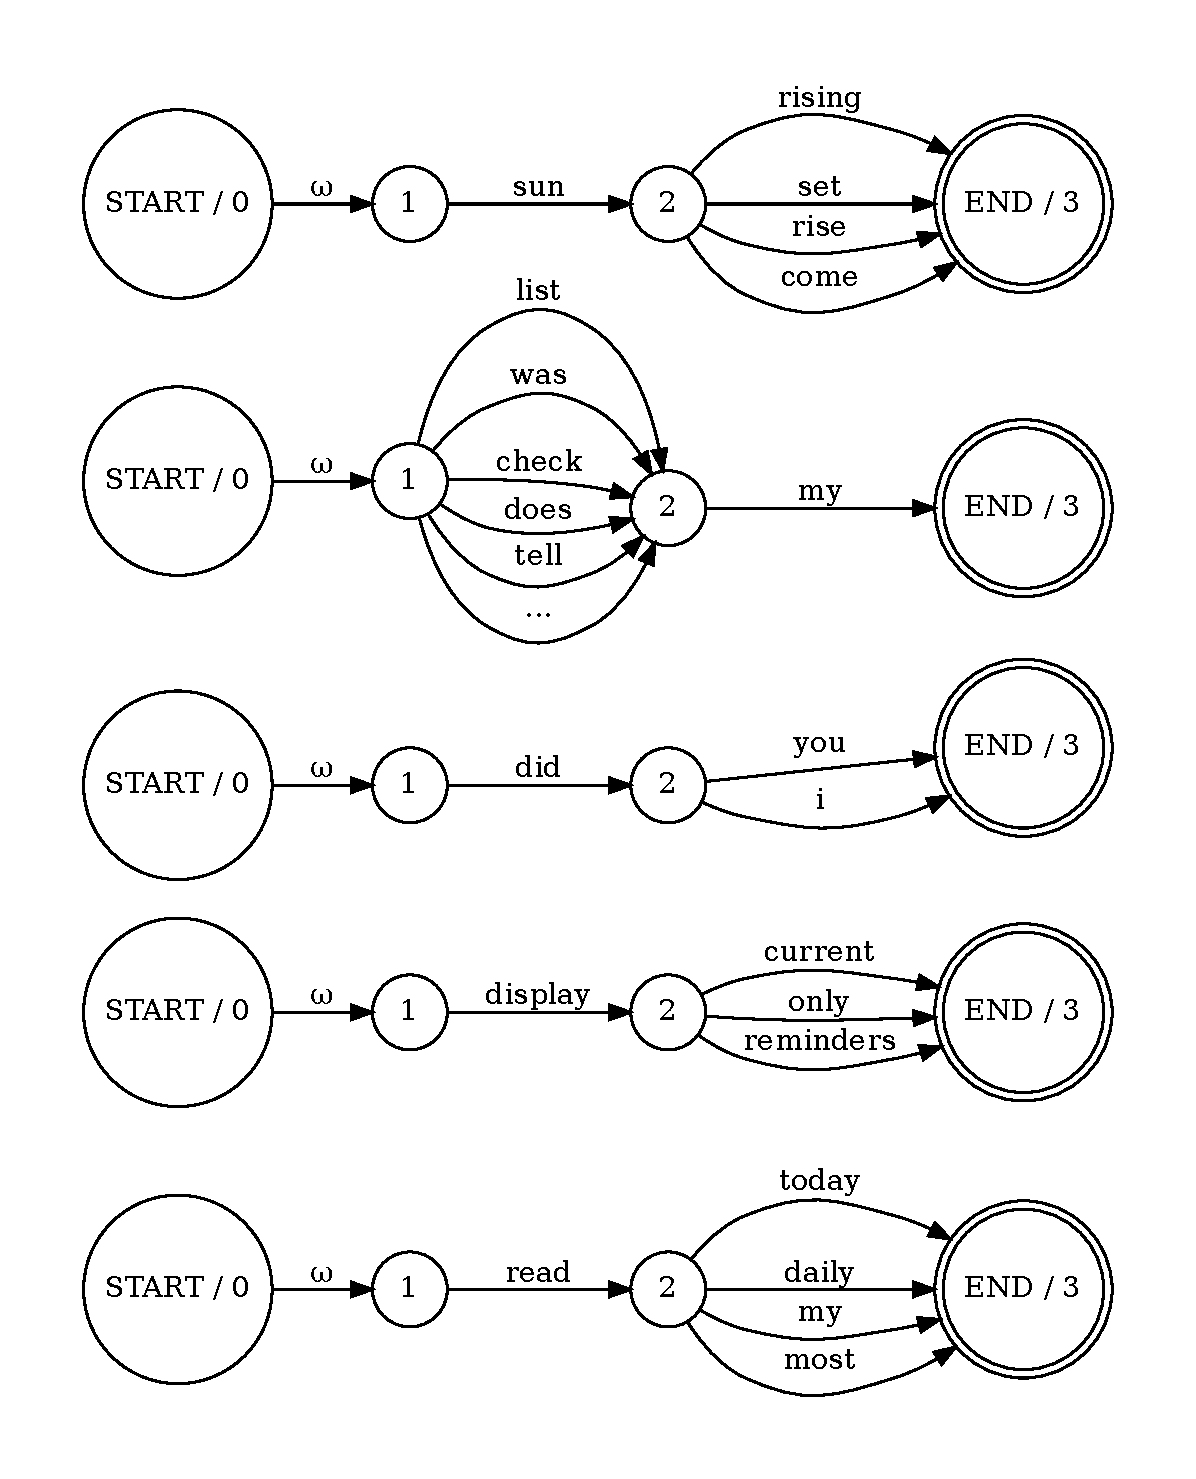
\includegraphics[trim={1.1cm 1.1cm 1.1cm
    1.1cm},clip,height=0.96\textheight]{pdfs/generated/neurons_regex_1618067722/activating_regex_sample_19.pdf}
  \caption[Ten sampled regular expressions from the RE lookup layer
  corresponding to TauSTE neuron 19 for the best performing small RE proxy
  model]{Ten sampled regular expressions from the RE lookup layer
    corresponding to TauSTE neuron 19 for the best performing small RE proxy
    model; REs are presented as equivalent NFAs; black signifies a
    main-path transition while blue signifies a $\omega$-transition}
  \label{fig:regex_example_neuron_alarm}
\end{figure}

\begin{figure}[t!]
  \centering
  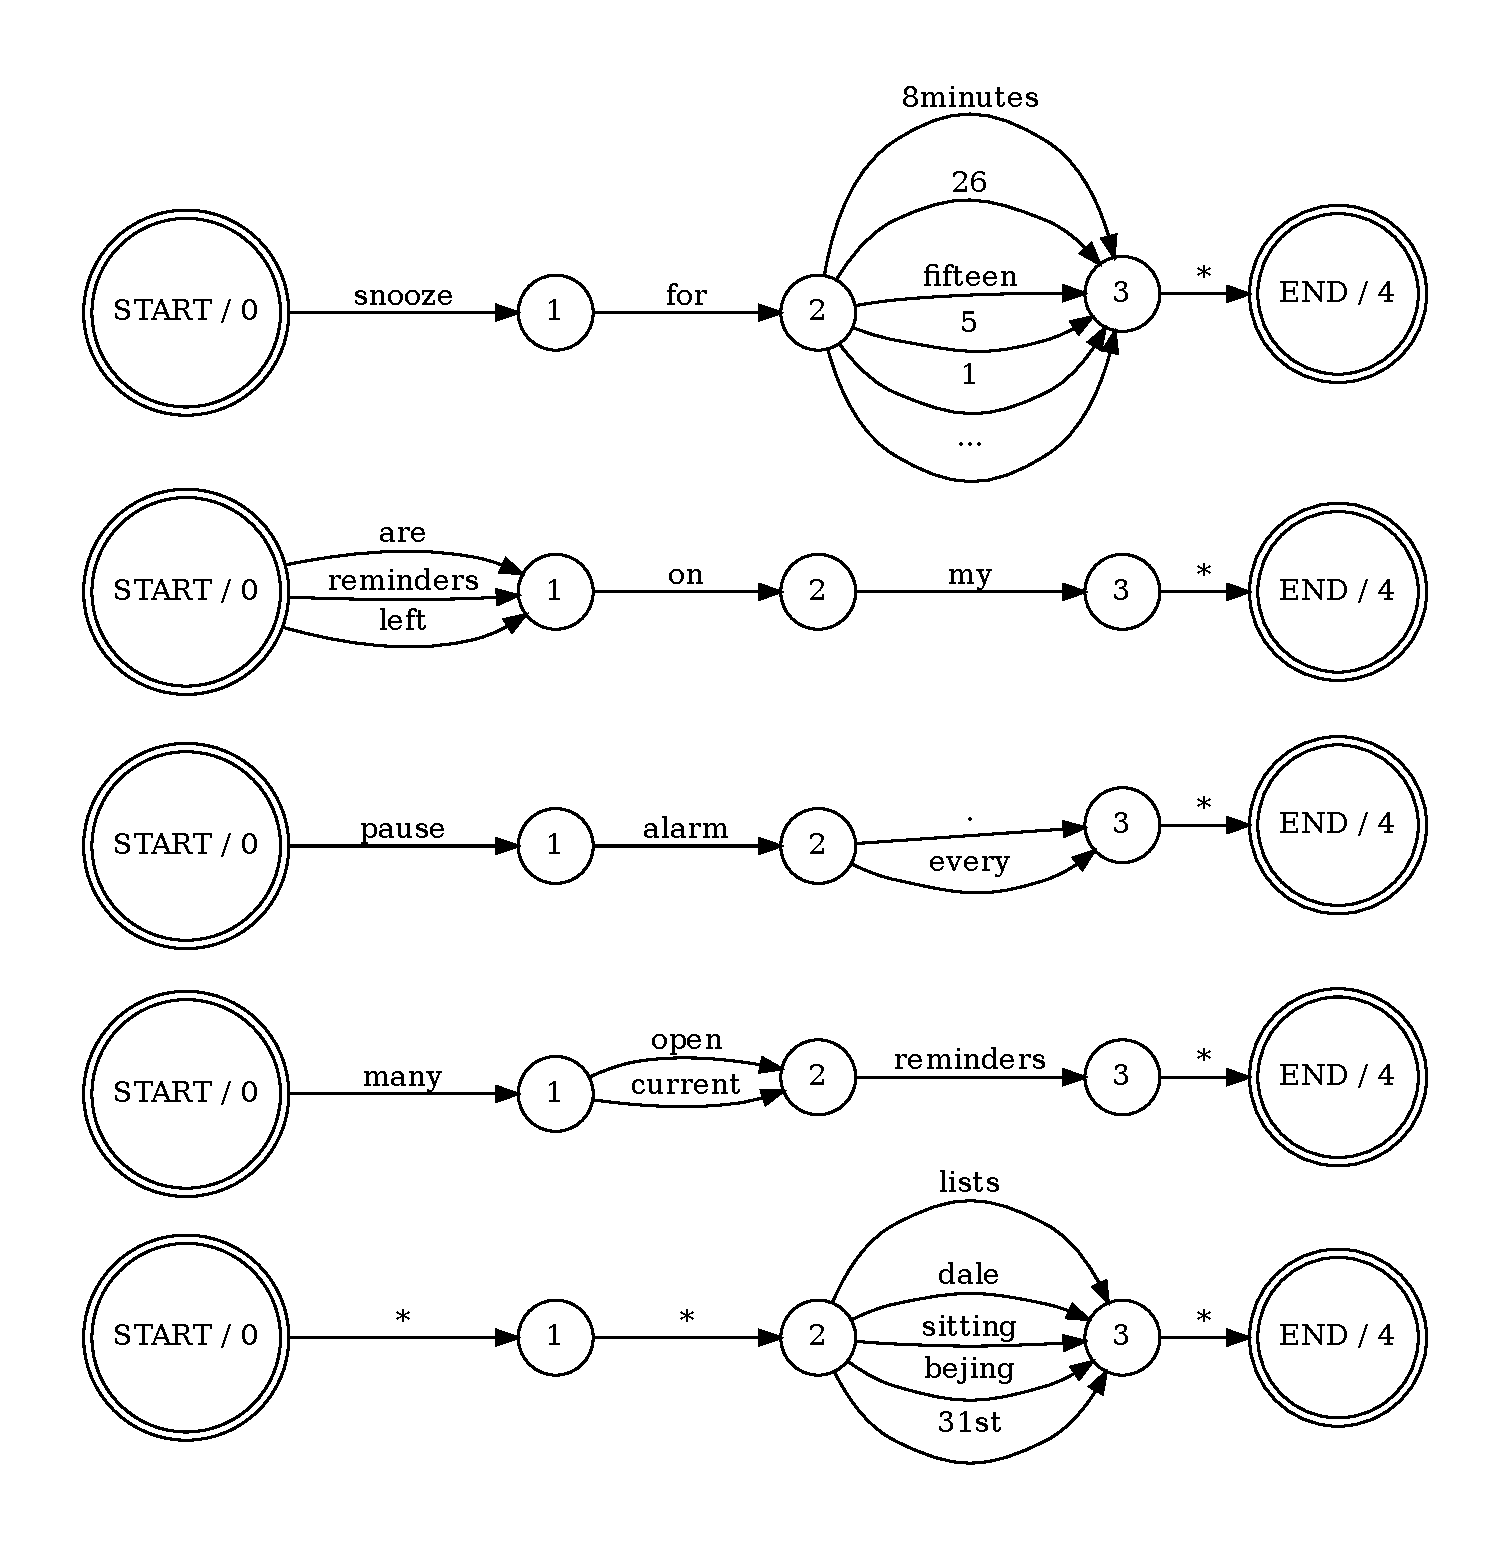
\includegraphics[trim={1.1cm 1.1cm 1.1cm 1.1cm},clip,height=0.96\textheight]{pdfs/generated/neurons_regex_1618067722/activating_regex_sample_25.pdf}
  \caption[Ten sampled regular expressions from the RE lookup layer
  corresponding to TauSTE neuron 25 for the best performing small RE proxy
  model]{Ten sampled regular expressions from the RE lookup layer
    corresponding to TauSTE neuron 25 for the best performing small RE proxy
    model; REs are presented as equivalent NFAs; black signifies a
    main-path transition while blue signifies a $\omega$-transition}
  \label{fig:regex_example_neuron_reminder}
\end{figure}

\begin{figure}[t!]
  \centering
  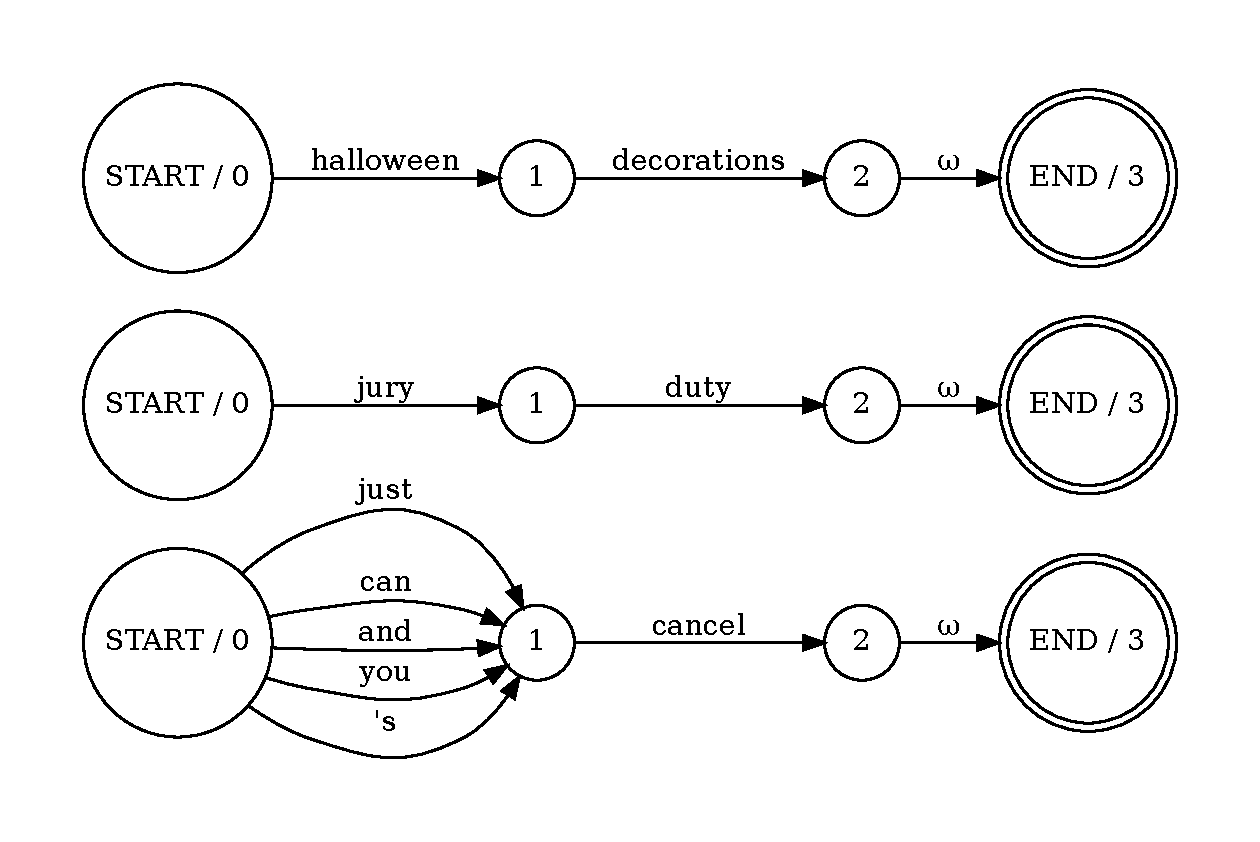
\includegraphics[trim={1.1cm 1.1cm 1.1cm 1.1cm},clip,height=0.96\textheight]{pdfs/generated/neurons_regex_1618067722/activating_regex_sample_17.pdf}
  \caption[Ten sampled regular expressions from the RE lookup layer
  corresponding to TauSTE neuron 17 for the best performing small RE proxy
  model]{Ten sampled regular expressions from the RE lookup layer
    corresponding to TauSTE neuron 17 for the best performing small RE proxy
    model; REs are presented as equivalent NFAs; black signifies a
    main-path transition while blue signifies a $\omega$-transition}
  \label{fig:regex_example_neuron_weather}
\end{figure}

\clearpage

%%% Local Variables: 
%%% mode: latex
%%% TeX-master: "main"
%%% End: 